\documentclass{article}
\usepackage[top=2.5cm, left=3cm, right=3cm, bottom=4.0cm]{geometry}
\usepackage{graphicx} 
\usepackage{amsfonts,amsmath,amssymb}
\usepackage{array}
\usepackage{tabularray}
\usepackage[utf8]{inputenc}
\usepackage[T1]{fontenc}
\usepackage{csquotes}
\usepackage{alphabeta}
\usepackage{tabularx}
\usepackage{url}
\usepackage{hyperref}
\usepackage{esint}

\renewcommand{\figurename}{Γράφημα}

\begin{document}
\begin{table}[ht]
    \begin{tblr}{
        @{}X[l, valign=b]X[c, valign=b]X[r, valign=b]@{}
    }

    \hline
    % First line, course info
    \SetCell[c=2]{l}{[ΘΠ04] Παράλληλα Συστήματα} & & {2024-25} \\ 
    \hline
    {} & {} & {} \\

    % Title
    \SetCell[c=3]{c}{ \Large \textbf{Εργασία 3 - Προγραμματισμός με MPI} } \\
    {} & {} & {} \\

    % Name Surname, Student ID
    \hline
    \SetCell[c=3]{c}{ \textbf{Ονοματεπώνυμο:} Μάριος Γιαννόπουλος } \\
    \SetCell[c=3]{c}{ \textbf{A.M.:} 1115200000032} \\
    \hline

    \end{tblr}
\end{table}
\section*{Γενικές Πληροφορίες}

\subsection*{Υπολογιστικό Σύστημα}
Όλο το έργο υλοποιήθηκε στο ίδιο υπολογιστικό περιβάλλον:
\begin{itemize}
    \item \textbf{Όνομα Υπολογιστικού Συστήματος:} Linux12
    \item \textbf{Επεξεργαστής:} Intel(R) Core(TM) i5-6500 CPU @ 3.20GHz
    \item \textbf{Αριθμός Πυρήνων:} 4
    \item \textbf{Λειτουργικό Σύστημα:} Linux Ubuntu 20.04.2 LTS
    \item \textbf{Έκδοση Μεταγλωττιστή:} gcc (Ubuntu 9.4.0-1ubuntu1~20.04.2) 9.4.0
\end{itemize}

\subsection*{Οδηγίες Εκτέλεσης Python Scripts}
Για την εκτέλεση των Python scripts που επεξεργάζονται τα αποτελέσματα, ακολουθήστε τα εξής βήματα:
\begin{enumerate}
    \item Μεταβείτε στον φάκελο \path{scripts}.
    \item Εγκαταστήστε τις απαραίτητες βιβλιοθήκες:
    \begin{verbatim}
    pip install -r requirements.txt
    \end{verbatim}
    \item Εκτελέστε το script που σας ενδιαφέρει:
    \begin{verbatim}
    python <test_script>.py
    \end{verbatim}
\end{enumerate}
\textbf{Σημείωση:} Όλα τα αποτελέσματα στα γραφήματα είναι από την εκτέλεση των πειραμάτων στο εργαστήριο Linux. Κάθε πείραμα εκτελέστηκε 5 φορές και τα αποτελέσματα αναφέρονται στο μέσο όρο των επαναλήψεων.
\section*{Άσκηση 3.1}
\subsection*{Εισαγωγή}
Το Παιχνίδι της Ζωής (Game of Life) είναι ένα κυτταρικό αυτόματο που αναπτύχθηκε από τον μαθηματικό John Horton Conway. Είναι ένα μοντέλο που προσομοιώνει την εξέλιξη ενός πληθυσμού κυττάρων σε ένα δισδιάστατο πλέγμα, όπου κάθε κύτταρο μπορεί να βρίσκεται σε μία από δύο καταστάσεις: ζωντανό ή νεκρό. 
Οι κανόνες που διέπουν την εξέλιξη του πληθυσμού βασίζονται στον αριθμό των γειτόνων κάθε κυττάρου.
Σε αυτή την άσκηση, υλοποιήθηκε μια παράλληλη έκδοση του Παιχνιδιού της Ζωής χρησιμοποιώντας την MPI (Message Passing Interface) για την κατανομή του υπολογιστικού φόρτου μεταξύ πολλαπλών διεργασιών. Η υλοποίηση βασίζεται στη σειριακή έκδοση του αλγορίθμου που αναπτύχθηκε στην Άσκηση 2.1, χωρίς τη χρήση OpenMP.
\subsection*{Συγχρονισμός}
Ο συγχρονισμός μεταξύ των διεργασιών είναι ένα κρίσιμο στοιχείο στην παράλληλη υλοποίηση του Παιχνιδιού της Ζωής. Στον κώδικα, ο συγχρονισμός επιτυγχάνεται με τις εξής λειτουργίες:
\begin{enumerate}
    \item \textbf{\path{MPI_Scatter}}: Η διεργασία 0 κατανέμει τα δεδομένα του πλέγματος στις υπόλοιπες διεργασίες.
    \item \textbf{\path{MPI_Sendrecv}}: Κάθε διεργασία ανταλλάσσει γραμμές ορίων (ghost rows) με τις γειτονικές της διεργασίες για να υπολογίσει σωστά την επόμενη γενιά.
    \item \textbf{\path{MPI_Gather}}: Η διεργασία 0 συγκεντρώνει τα αποτελέσματα από όλες τις διεργασίες για να ενημερώσει το τελικό πλέγμα.
\end{enumerate}
Αυτές οι λειτουργίες εξασφαλίζουν ότι οι διεργασίες συνεργάζονται αποτελεσματικά και ότι τα δεδομένα παραμένουν συνεπή κατά τη διάρκεια της εκτέλεσης.
\subsection*{Πειραματική Διαδικασία}
\begin{itemize}
    \item \textbf{Παραμετροποίηση:}
    \begin{itemize}
        \item Μέγεθος πλέγματος: $64 \times 64$, $1024 \times 1024$, $4096 \times 4096$.
        \item Αριθμός διεργασιών: 2, 4, 8, 16.
        \item Αριθμός γενιών: 1000.
    \end{itemize}
    \item \textbf{Εκτέλεση:}
    \begin{itemize}
        \item Τα πειράματα εκτελέστηκαν 5 φορές για κάθε συνδυασμό παραμέτρων.
        \item Καταγράφηκε ο χρόνος εκτέλεσης για κάθε πείραμα.
        \item Τα δεδομένα αποθηκεύτηκαν σε CSV αρχείο.
    \end{itemize}
    \item \textbf{Αυτοματοποίηση:}
    \begin{itemize}
        \item Αναπτύχθηκαν Python scripts για την εκτέλεση των πειραμάτων και την καταγραφή των δεδομένων.
        \item Χρησιμοποιήθηκαν Python scripts για την επεξεργασία των αποτελεσμάτων και τη δημιουργία γραφημάτων.
    \end{itemize}
\end{itemize}
\subsection*{Αποτελέσματα}
Από τα αποτελέσματα των μετρήσεων, παρατηρούμε τα εξής:
\begin{enumerate}
    \item \textbf{Για μικρά μεγέθη πλέγματος (64x64)}:
    \begin{itemize}
        \item Η χρήση περισσότερων διεργασιών δεν οδηγεί πάντα σε μείωση του χρόνου εκτέλεσης. Για παράδειγμα, η χρήση 4 διεργασιών οδήγησε σε μεγαλύτερο χρόνο εκτέλεσης (2.20885 s) σε σύγκριση με τη χρήση 2 διεργασιών (1.72495 s). Αυτό οφείλεται στο γεγονός ότι το κόστος επικοινωνίας μεταξύ των διεργασιών είναι υψηλό σε σχέση με τον χρόνο υπολογισμού για τόσο μικρά πλέγματα.
        \item Η χρήση 8 και 16 διεργασιών οδήγησε σε ακόμη μεγαλύτερους χρόνους εκτέλεσης (7.92210 s και 10.79159 s αντίστοιχα), γεγονός που επιβεβαιώνει ότι για μικρά πλέγματα η παράλληλη εκτέλεση δεν είναι αποτελεσματική.
    \end{itemize}
    \item \textbf{Για μεσαία μεγέθη πλέγματος (1024x1024)}:
    \begin{itemize}
        \item Η χρήση 4 διεργασιών οδήγησε σε σημαντική μείωση του χρόνου εκτέλεσης (7.71714 s) σε σύγκριση με τη χρήση 2 διεργασιών (21.93556 s). Αυτό δείχνει ότι για μεσαία μεγέθη πλέγματος, η παράλληλη εκτέλεση αρχίζει να γίνεται αποτελεσματική.
        \item Ωστόσο, η χρήση 8 και 16 διεργασιών οδήγησε σε αύξηση του χρόνου εκτέλεσης (22.11091 s και 16.76202 s αντίστοιχα), γεγονός που υποδηλώνει ότι το κόστος επικοινωνίας αρχίζει να γίνεται σημαντικό για μεγαλύτερο αριθμό διεργασιών.
    \end{itemize}
    \item \textbf{Για μεγάλα μεγέθη πλέγματος (4096x4096)}:
    \begin{itemize}
        \item Η χρήση περισσότερων διεργασιών οδήγησε σε σημαντική μείωση του χρόνου εκτέλεσης. Για παράδειγμα, η χρήση 16 διεργασιών οδήγησε σε μέσο χρόνο εκτέλεσης 75.97231 s, σε σύγκριση με 425.03920 s για 2 διεργασίες.
        \item Αυτό δείχνει ότι για πολύ μεγάλα πλέγματα, η παράλληλη εκτέλεση είναι πολύ αποτελεσματική, καθώς ο χρόνος υπολογισμού κυριαρχεί έναντι του χρόνου επικοινωνίας.
    \end{itemize}
\end{enumerate}
\subsection*{Γραφήματα}
\begin{figure}[h]
    \centering
    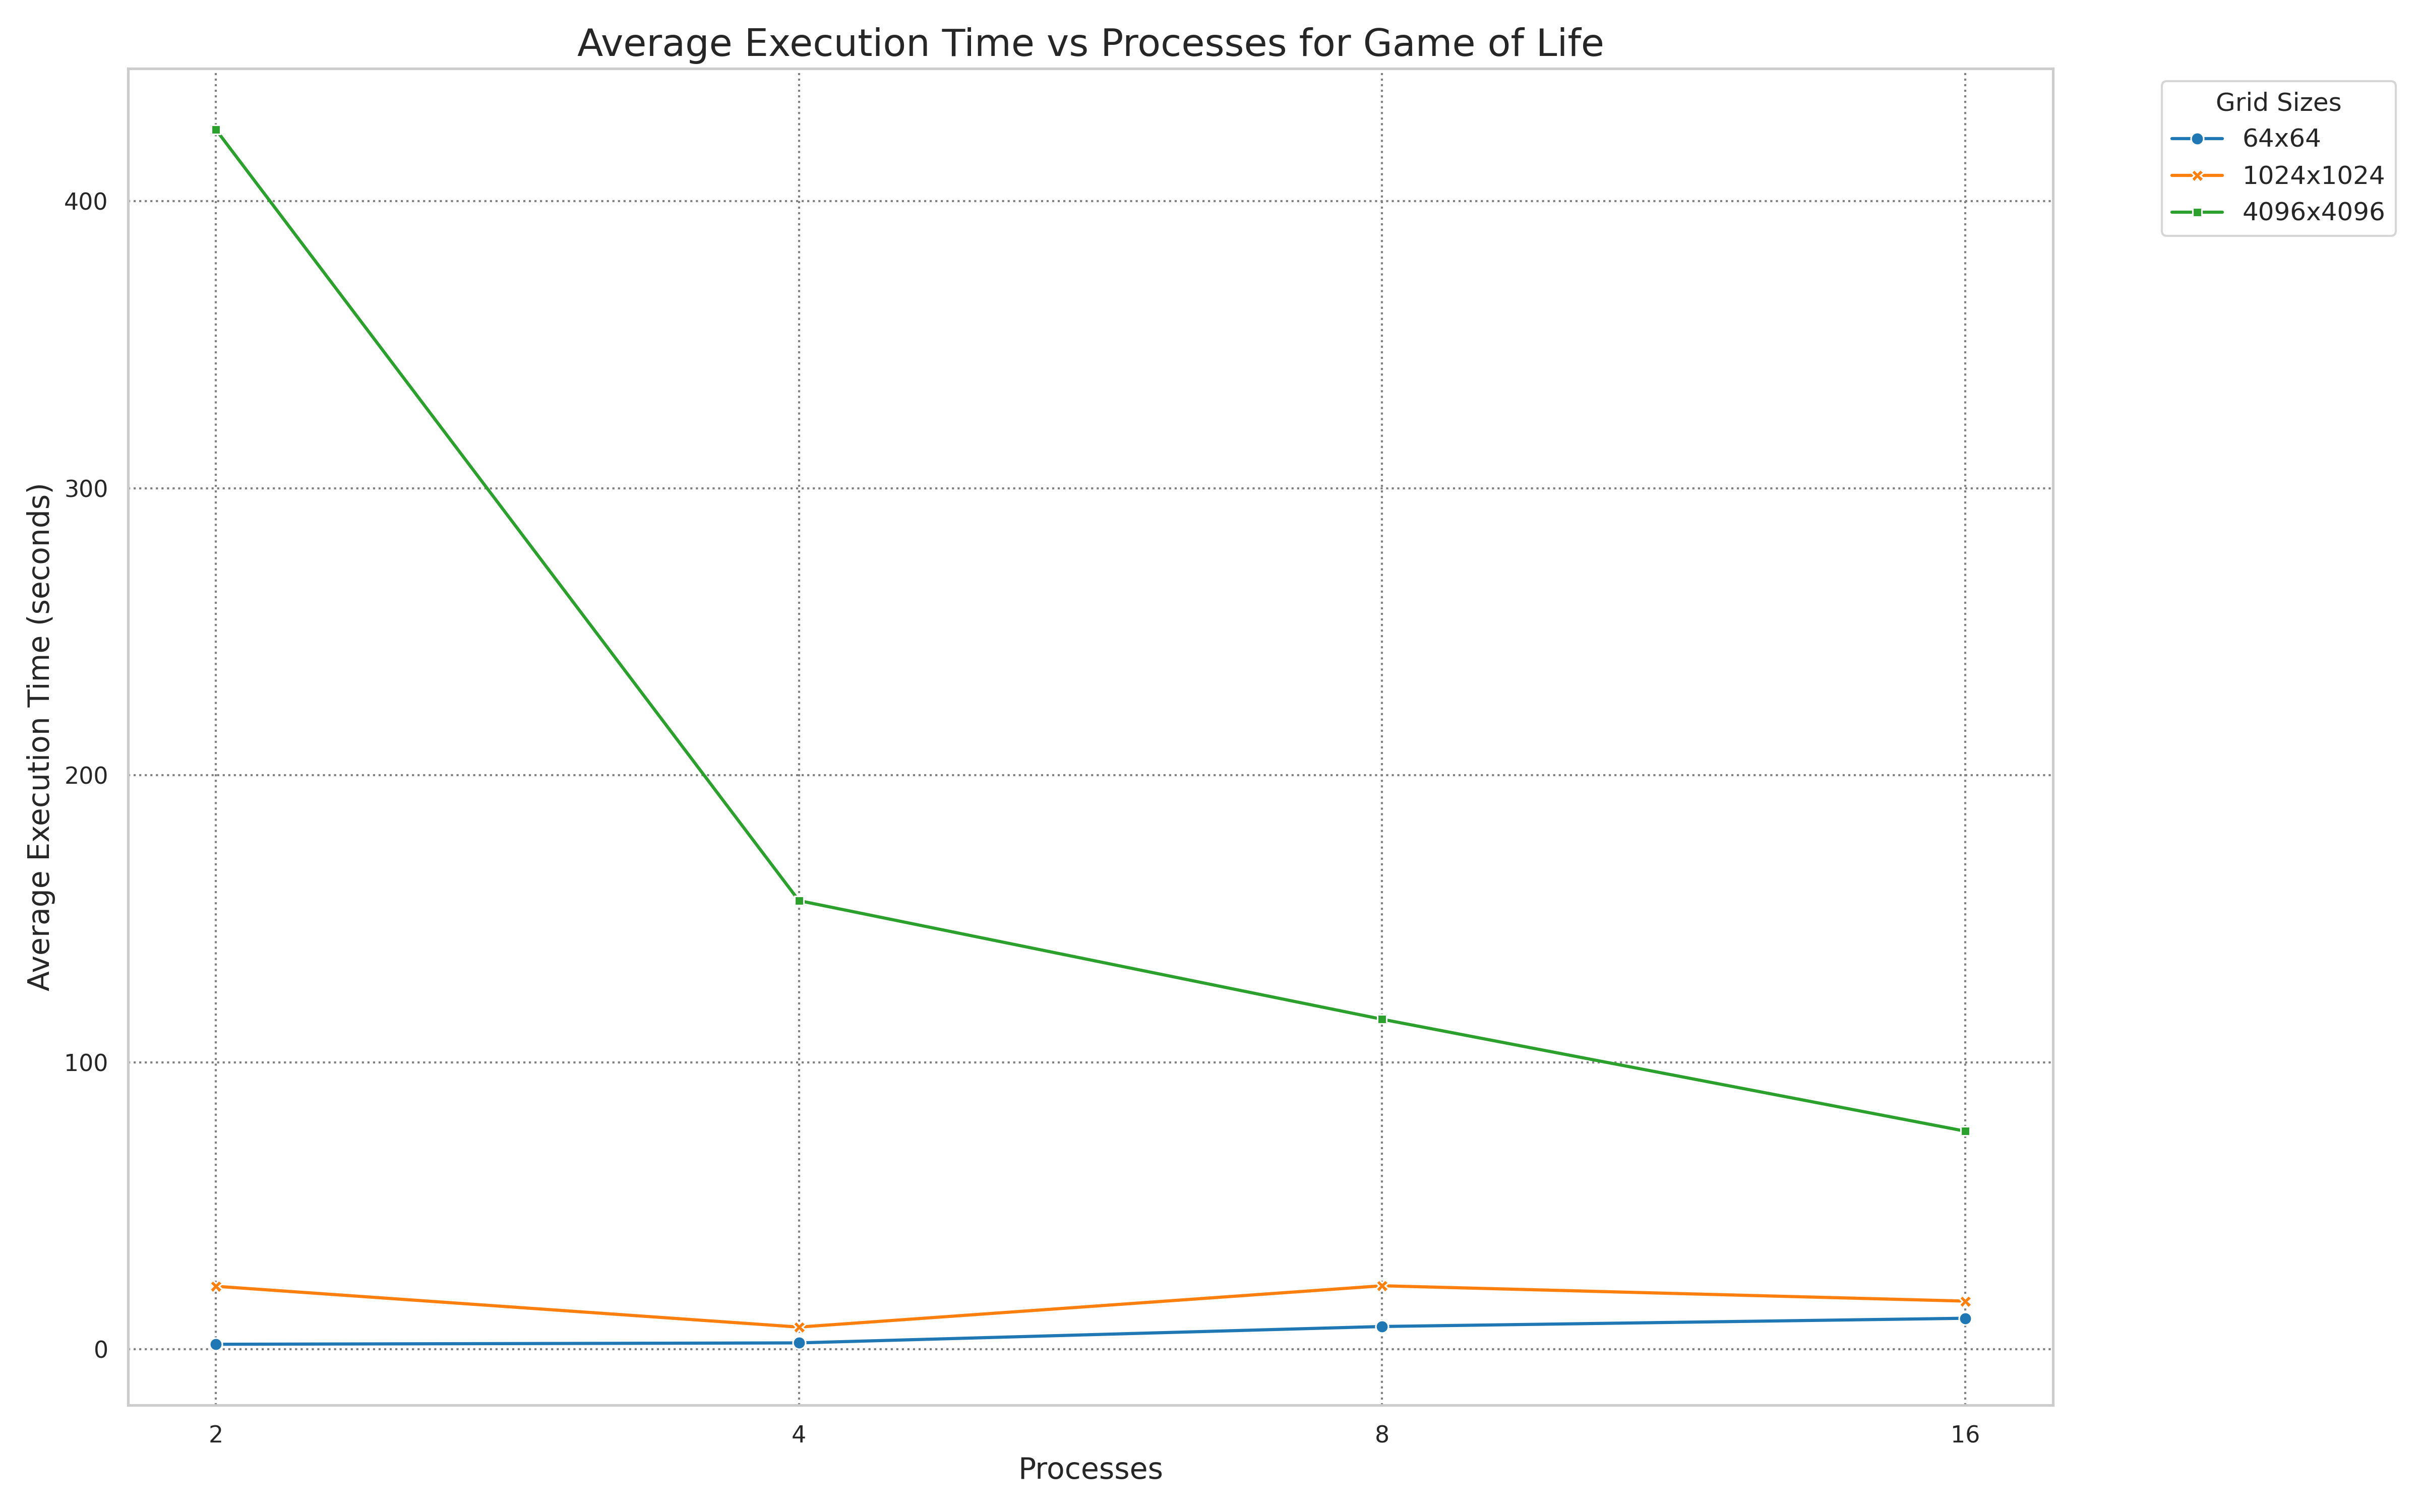
\includegraphics[width=0.8\textwidth]{game_of_life_mpi_results.png}
    \caption{Χρόνοι εκτέλεσης για το Παιχνίδι της Ζωής με MPI}
\end{figure}
\subsection*{Συμπεράσματα}
Από τα αποτελέσματα και τα γραφήματα, μπορούμε να εξάγουμε τα εξής συμπεράσματα:
\begin{enumerate}
    \item \textbf{Επίδραση του μεγέθους πλέγματος}:
    \begin{itemize}
        \item Για μικρά μεγέθη πλέγματος, η παράλληλη εκτέλεση δεν είναι αποτελεσματική λόγω του υψηλού κόστους επικοινωνίας σε σχέση με τον χρόνο υπολογισμού.
        \item Για μεσαία και μεγάλα μεγέθη πλέγματος, η παράλληλη εκτέλεση γίνεται ολοένα και πιο αποτελεσματική, καθώς ο χρόνος υπολογισμού κυριαρχεί έναντι του χρόνου επικοινωνίας.
    \end{itemize}
    \item \textbf{Επίδραση του αριθμού των διεργασιών}:
    \begin{itemize}
        \item Για μικρά πλέγματα, η αύξηση του αριθμού των διεργασιών οδηγεί σε αύξηση του χρόνου εκτέλεσης λόγω του κόστους επικοινωνίας.
        \item Για μεγάλα πλέγματα, η αύξηση του αριθμού των διεργασιών οδηγεί σε σημαντική μείωση του χρόνου εκτέλεσης, καθώς ο χρόνος υπολογισμού είναι πολύ μεγαλύτερος από το κόστος επικοινωνίας.
    \end{itemize}
    \item \textbf{Βέλτιστος αριθμός διεργασιών}:
    \begin{itemize}
        \item Για κάθε μέγεθος πλέγματος, υπάρχει ένας βέλτιστος αριθμός διεργασιών που εξαρτάται από το μέγεθος του πλέγματος και το κόστος επικοινωνίας. Για παράδειγμα, για πλέγμα 1024x1024, ο βέλτιστος αριθμός διεργασιών φαίνεται να είναι 4, ενώ για πλέγμα 4096x4096, ο βέλτιστος αριθμός διεργασιών φαίνεται να είναι 16.
    \end{itemize}
\end{enumerate}
Συνολικά, η παράλληλη υλοποίηση του Παιχνιδιού της Ζωής με MPI αποδεικνύεται πολύ αποτελεσματική για μεγάλα προβλήματα, ενώ για μικρά προβλήματα η σειριακή εκτέλεση μπορεί να είναι επαρκής. Η επιλογή του βέλτιστου αριθμού διεργασιών εξαρτάται από το μέγεθος του πλέγματος και το κόστος επικοινωνίας μεταξύ των διεργασιών.
\section*{Άσκηση 3.2}
\subsection*{Εισαγωγή}
Ο πολλαπλασιασμός πίνακα-διανύσματος είναι μια θεμελιώδης πράξη στη γραμμική άλγεβρα, η οποία βρίσκει εφαρμογές σε πολλούς τομείς όπως η επιστήμη των υπολογιστών, η φυσική και η μηχανική. Σε αυτή την άσκηση, υλοποιήθηκε ένα παράλληλο πρόγραμμα χρησιμοποιώντας την MPI (Message Passing Interface) για τον υπολογισμό του πολλαπλασιασμού πίνακα-διανύσματος με κατανομή του πίνακα κατά μπλοκ-στήλες. Η υλοποίηση βασίζεται στη σειριακή έκδοση του αλγορίθμου, όπου η διεργασία 0 δημιουργεί τον πίνακα και το διάνυσμα και κατανέμει τα δεδομένα στις υπόλοιπες διεργασίες για παράλληλο υπολογισμό.
\subsection*{Συγχρονισμός}
Ο συγχρονισμός μεταξύ των διεργασιών είναι ένα κρίσιμο στοιχείο στην παράλληλη υλοποίηση του πολλαπλασιασμού πίνακα-διανύσματος. Στον κώδικα, ο συγχρονισμός επιτυγχάνεται με τις εξής λειτουργίες:
\begin{enumerate}
    \item \textbf{\path{MPI_Scatter}}: Η διεργασία 0 κατανέμει τις στήλες του πίνακα στις υπόλοιπες διεργασίες.
    \item \textbf{\path{MPI_Bcast}}: Η διεργασία 0 μεταδίδει το διάνυσμα σε όλες τις διεργασίες.
    \item \textbf{\path{MPI_Reduce}}: Οι διεργασίες στέλνουν τα τοπικά αποτελέσματα στη διεργασία 0, όπου συγκεντρώνονται για τον τελικό υπολογισμό.
\end{enumerate}
Αυτές οι λειτουργίες εξασφαλίζουν ότι οι διεργασίες συνεργάζονται αποτελεσματικά και ότι τα δεδομένα παραμένουν συνεπή κατά τη διάρκεια της εκτέλεσης.
\subsection*{Πειραματική Διαδικασία}
\begin{itemize}
    \item \textbf{Παραμετροποίηση:}
    \begin{itemize}
        \item Μέγεθος πίνακα: $100\times100$, $1000\times1000$, $5000\times5000$, $10000\times10000$.
        \item Αριθμός διεργασιών: 2, 4, 5, 10.
    \end{itemize}
    \item \textbf{Εκτέλεση:}
    \begin{itemize}
        \item Τα πειράματα εκτελέστηκαν 5 φορές για κάθε συνδυασμό παραμέτρων.
        \item Καταγράφηκε ο χρόνος εκτέλεσης για κάθε πείραμα.
        \item Τα δεδομένα αποθηκεύτηκαν σε CSV αρχείο.
    \end{itemize}
    \item \textbf{Αυτοματοποίηση:}
    \begin{itemize}
        \item Αναπτύχθηκαν Python scripts για την εκτέλεση των πειραμάτων και την καταγραφή των δεδομένων.
        \item Χρησιμοποιήθηκαν Python scripts για την επεξεργασία των αποτελεσμάτων και τη δημιουργία γραφημάτων.
    \end{itemize}
\end{itemize}
\subsection*{Αποτελέσματα}
Σε αυτή την ενότητα, παρουσιάζονται τα αποτελέσματα των χρόνων εκτέλεσης για τον πολλαπλασιασμό πίνακα-διανύσματος με βάση τα δεδομένα που παρέχονται. Οι χρόνοι εκτέλεσης καταγράφηκαν για διαφορετικούς αριθμούς διεργασιών (2, 4, 5, 10) και διαφορετικά μεγέθη πινάκων (100x100, 1000x1000, 5000x5000, 10000x10000). Τα αποτελέσματα παρουσιάζονται σε μορφή πίνακα και αναλύονται παρακάτω.
\subsubsection*{Πίνακας Χρόνων Εκτέλεσης}
\begin{table}[h]
\centering
\begin{tabularx}{\textwidth}{|c|c|c|X|}
    \hline
    \textbf{Διεργασίες} & \textbf{Μέγεθος Πίνακα} & \textbf{Χρόνος (s)} & \textbf{Παρατηρήσεις} \\
    \hline
    2 & 100x100 & 1.43 & - \\
    2 & 1000x1000 & 3.02 & - \\
    2 & 5000x5000 & 38.35 & - \\
    2 & 10000x10000 & 150.54 & - \\
    \hline
    4 & 100x100 & 1.49 & Χαμηλή βελτίωση σε σχέση με 2 διεργασίες \\
    4 & 1000x1000 & 3.79 & Αύξηση του χρόνου λόγω επικοινωνίας \\
    4 & 5000x5000 & 59.94 & Αύξηση του χρόνου σε σχέση με 2 διεργασίες \\
    4 & 10000x10000 & 230.98 & Αύξηση του χρόνου σε σχέση με 2 διεργασίες \\
    \hline
    5 & 100x100 & 1.55 & Χαμηλή βελτίωση σε σχέση με 2 διεργασίες \\
    5 & 1000x1000 & 4.01 & Αύξηση του χρόνου λόγω επικοινωνίας \\
    5 & 5000x5000 & 58.86 & Μικρή βελτίωση σε σχέση με 4 διεργασίες \\
    5 & 10000x10000 & 236.74 & Μικρή βελτίωση σε σχέση με 4 διεργασίες \\
    \hline
    10 & 100x100 & 1.58 & Χαμηλή βελτίωση σε σχέση με 2 διεργασίες \\
    10 & 1000x1000 & 3.94 & Αύξηση του χρόνου λόγω επικοινωνίας \\
    10 & 5000x5000 & 60.55 & Αύξηση του χρόνου σε σχέση με 2 διεργασίες \\
    10 & 10000x10000 & 234.36 & Μικρή βελτίωση σε σχέση με 4 διεργασίες \\
    \hline
\end{tabularx}
\caption{Σύγκριση χρόνων εκτέλεσης για διαφορετικούς αριθμούς διεργασιών και μεγέθη πινάκων}
\end{table}
\subsubsection*{Ανάλυση Αποτελεσμάτων}
\begin{enumerate}
    \item \textbf{Για μικρούς πίνακες (100x100)}:
    \begin{itemize}
        \item Η χρήση περισσότερων διεργασιών δεν οδηγεί σε σημαντική μείωση του χρόνου εκτέλεσης. Για παράδειγμα, η χρήση 10 διεργασιών οδήγησε σε μέσο χρόνο εκτέλεσης 1.582433 s, σε σύγκριση με 1.429126 s για 2 διεργασίες. Αυτό οφείλεται στο γεγονός ότι το κόστος επικοινωνίας μεταξύ των διεργασιών είναι υψηλό σε σχέση με τον χρόνο υπολογισμού για τόσο μικρούς πίνακες.
    \end{itemize}
    \item \textbf{Για μεσαίους πίνακες (1000x1000)}:
    \begin{itemize}
        \item Η χρήση περισσότερων διεργασιών οδηγεί σε αύξηση του χρόνου εκτέλεσης. Για παράδειγμα, η χρήση 10 διεργασιών οδήγησε σε μέσο χρόνο εκτέλεσης 3.938691 s, σε σύγκριση με 3.018212 s για 2 διεργασίες. Αυτό υποδηλώνει ότι το κόστος επικοινωνίας αρχίζει να γίνεται σημαντικό για μεγαλύτερο αριθμό διεργασιών.
    \end{itemize}
    \item \textbf{Για μεγάλους πίνακες (5000x5000 και 10000x10000)}:
    \begin{itemize}
        \item Η χρήση περισσότερων διεργασιών δεν οδηγεί σε σημαντική μείωση του χρόνου εκτέλεσης. Για παράδειγμα, για πίνακα 5000x5000, η χρήση 10 διεργασιών οδήγησε σε μέσο χρόνο εκτέλεσης 60.547491 s, σε σύγκριση με 38.354262 s για 2 διεργασίες. Αυτό δείχνει ότι για πολύ μεγάλους πίνακες, το κόστος επικοινωνίας είναι υψηλό και η παράλληλη εκτέλεση δεν είναι πάντα αποτελεσματική.
    \end{itemize}
    \item \textbf{Βέλτιστος αριθμός διεργασιών}:
    \begin{itemize}
        \item Για μικρούς πίνακες, ο βέλτιστος αριθμός διεργασιών φαίνεται να είναι 2, καθώς η χρήση περισσότερων διεργασιών οδηγεί σε αύξηση του χρόνου εκτέλεσης λόγω του κόστους επικοινωνίας.
        \item Για μεσαίους πίνακες, ο βέλτιστος αριθμός διεργασιών φαίνεται να είναι επίσης 2, καθώς η χρήση περισσότερων διεργασιών οδηγεί σε αύξηση του χρόνου εκτέλεσης.
        \item Για μεγάλους πίνακες, ο βέλτιστος αριθμός διεργασιών εξαρτάται από το κόστος επικοινωνίας και τον χρόνο υπολογισμού. Ωστόσο, από τα δεδομένα, φαίνεται ότι η χρήση 2 διεργασιών είναι η πιο αποτελεσματική.
    \end{itemize}
\end{enumerate}
\subsection*{Γραφήματα}
\newpage
\begin{figure}[h]
    \centering
    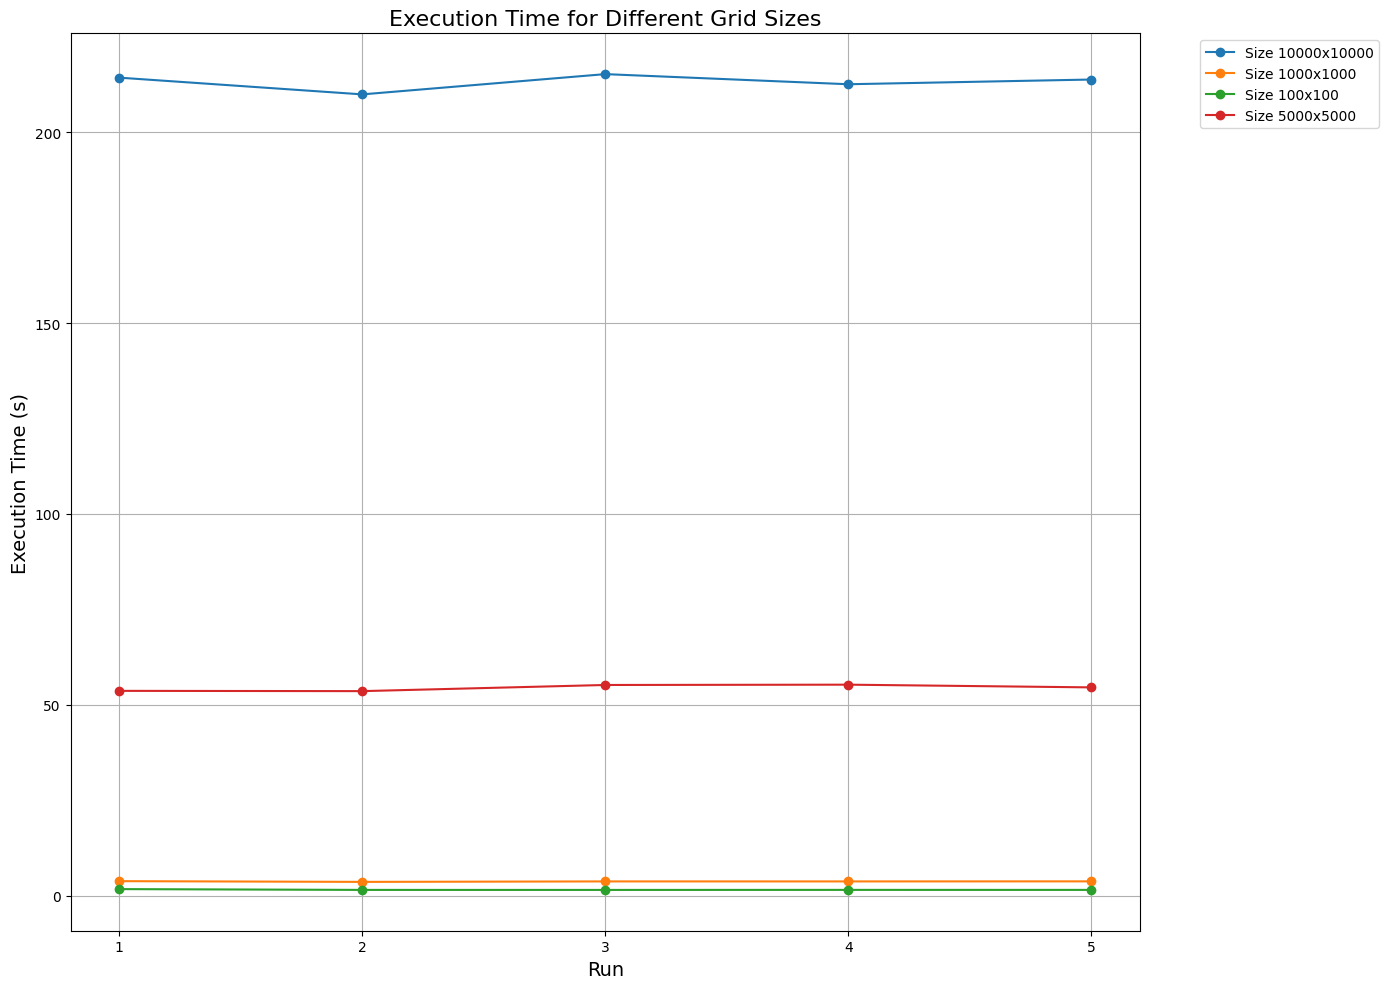
\includegraphics[width=0.8\textwidth]{matrix_vector_mpi_results.png}
    \caption{Χρόνοι εκτέλεσης για τον Πολλαπλασιασμό Πίνακα-Διανύσματος με MPI}
\end{figure}
\begin{figure}[h]
    \centering
    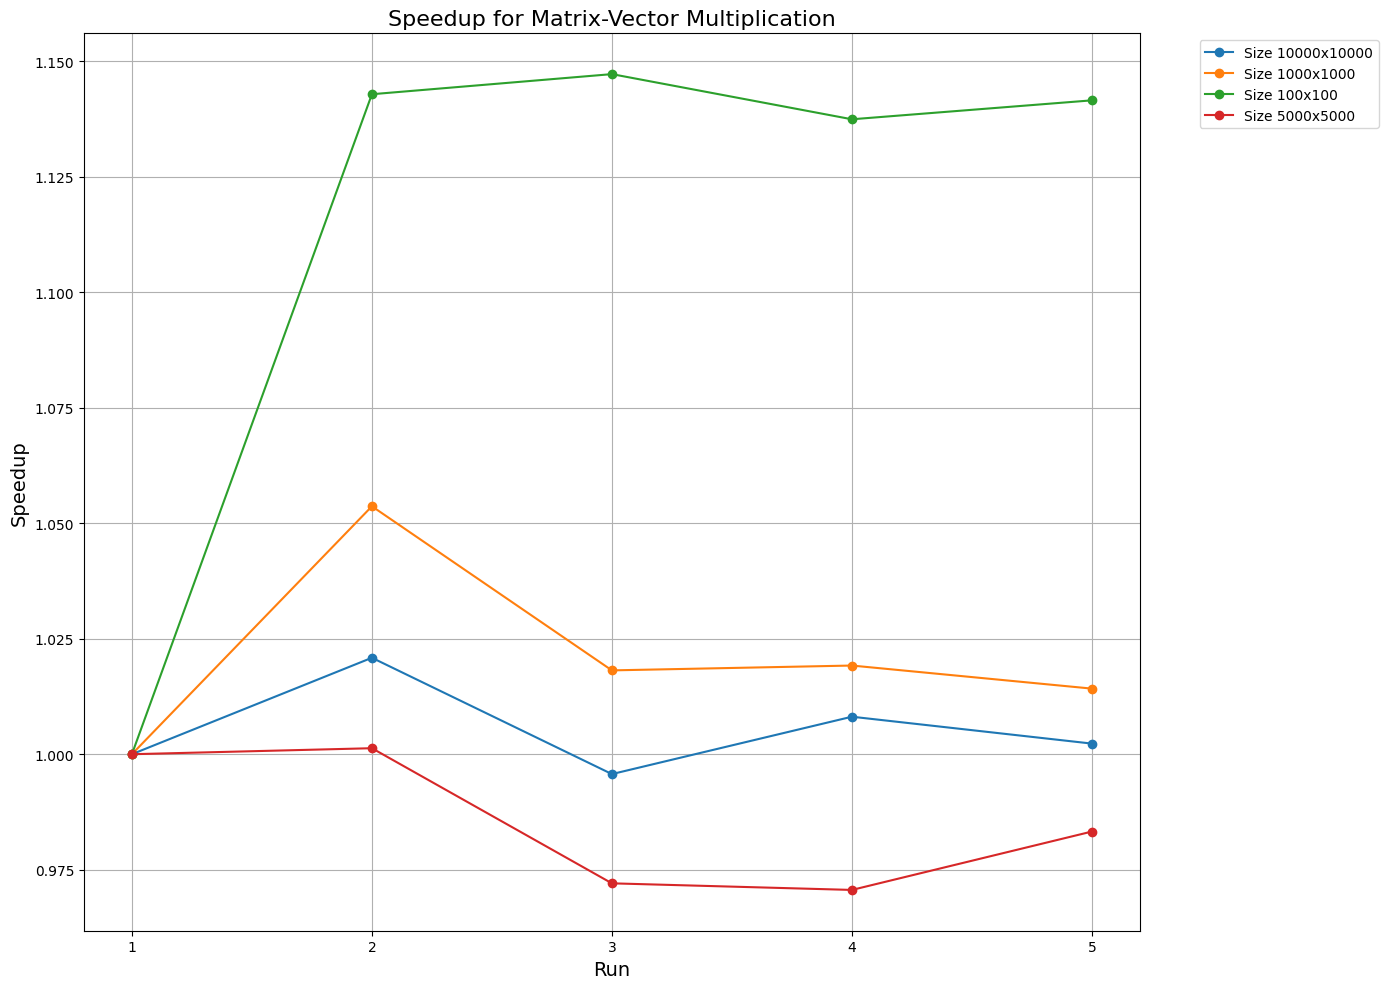
\includegraphics[width=0.8\textwidth]{matrix_vector_multiplication_speedup.png}
    \caption{Επιτάχυνση για τον Πολλαπλασιασμό Πίνακα-Διανύσματος με MPI}
\end{figure}
\newpage
\subsection*{Συμπεράσματα}
Από τα αποτελέσματα και τα γραφήματα, μπορούμε να εξάγουμε τα εξής συμπεράσματα:
\begin{enumerate}
    \item \textbf{Για μικρούς πίνακες (100x100)}:
    \begin{itemize}
        \item Η χρήση περισσότερων διεργασιών δεν οδηγεί σε σημαντική μείωση του χρόνου εκτέλεσης λόγω του υψηλού κόστους επικοινωνίας σε σχέση με τον χρόνο υπολογισμού.
    \end{itemize}
    \item \textbf{Για μεσαίους πίνακες (1000x1000)}:
    \begin{itemize}
        \item Η χρήση περισσότερων διεργασιών οδηγεί σε αύξηση του χρόνου εκτέλεσης λόγω του κόστους επικοινωνίας.
    \end{itemize}
    \item \textbf{Για μεγάλους πίνακες (5000x5000 και 10000x10000)}:
    \begin{itemize}
        \item Η χρήση περισσότερων διεργασιών δεν οδηγεί σε σημαντική μείωση του χρόνου εκτέλεσης, καθώς το κόστος επικοινωνίας είναι υψηλό.
    \end{itemize}
    \item \textbf{Βέλτιστος αριθμός διεργασιών}:
    \begin{itemize}
        \item Για όλα τα μεγέθη πινάκων, η χρήση 2 διεργασιών φαίνεται να είναι η πιο αποτελεσματική, καθώς η αύξηση του αριθμού των διεργασιών οδηγεί σε αύξηση του χρόνου εκτέλεσης λόγω του κόστους επικοινωνίας.
    \end{itemize}
\end{enumerate}
Συνολικά, η παράλληλη υλοποίηση του πολλαπλασιασμού πίνακα-διανύσματος με MPI αποδεικνύεται πιο αποτελεσματική για μικρούς και μεσαίους πίνακες όταν χρησιμοποιούνται 2 διεργασίες. Για μεγάλους πίνακες, η αύξηση του αριθμού των διεργασιών δεν οδηγεί σε σημαντική μείωση του χρόνου εκτέλεσης λόγω του υψηλού κόστους επικοινωνίας.
\section*{Άσκηση 3.3}
\subsection*{Εισαγωγή}
Σε αυτή την άσκηση, τροποποιήθηκε η παράλληλη υλοποίηση του Παιχνιδιού της Ζωής από την Άσκηση 3.1, ώστε να υπάρχει χρονική επικάλυψη μεταξύ των υπολογισμών και των επικοινωνιών. Αυτό επιτεύχθηκε με τη χρήση των ασύγχρονων MPI συναρτήσεων \texttt{\path{MPI_Isend()}}, \texttt{\path{MPI_Irecv()}} και \texttt{\path{MPI_Wait()}}. Η χρονική επικάλυψη επιτρέπει την ταυτόχρονη εκτέλεση υπολογισμών και επικοινωνιών, γεγονός που μπορεί να βελτιώσει την απόδοση του προγράμματος, ειδικά σε περιπτώσεις όπου ο χρόνος επικοινωνίας είναι σημαντικός.
\subsection*{Συγχρονισμός και Επικοινωνία}
Ο συγχρονισμός μεταξύ των διεργασιών εξακολουθεί να είναι κρίσιμος, αλλά τώρα επιτυγχάνεται με ασύγχρονες επικοινωνίες. Οι κύριες λειτουργίες που χρησιμοποιούνται είναι:
\begin{enumerate}
    \item \textbf{\texttt{\path{MPI_Isend()}}}: Αποστέλλει ασύγχρονα τα δεδομένα των γραμμών ορίων (ghost rows) στις γειτονικές διεργασίες.
    \item \textbf{\texttt{\path{MPI_Irecv()}}}: Λαμβάνει ασύγχρονα τα δεδομένα από τις γειτονικές διεργασίες.
    \item \textbf{\texttt{\path{MPI_Wait()}}}: Εξασφαλίζει ότι οι επικοινωνίες έχουν ολοκληρωθεί πριν προχωρήσουμε στον επόμενο υπολογισμό.
\end{enumerate}
\subsection*{Πειραματική Διαδικασία}
\begin{itemize}
    \item \textbf{Παραμετροποίηση:}
    \begin{itemize}
        \item Μέγεθος πλέγματος: $64 \times 64$, $1024 \times 1024$, $4096 \times 4096$.
        \item Αριθμός διεργασιών: 2, 4, 8, 16.
        \item Αριθμός γενιών: 1000.
    \end{itemize}
    \item \textbf{Εκτέλεση:}
    \begin{itemize}
        \item Τα πειράματα εκτελέστηκαν 5 φορές για κάθε συνδυασμό παραμέτρων.
        \item Καταγράφηκε ο χρόνος εκτέλεσης για κάθε πείραμα.
        \item Τα δεδομένα αποθηκεύτηκαν σε CSV αρχείο.
    \end{itemize}
    \item \textbf{Αυτοματοποίηση:}
    \begin{itemize}
        \item Αναπτύχθηκαν Python scripts για την εκτέλεση των πειραμάτων και την καταγραφή των δεδομένων.
        \item Χρησιμοποιήθηκαν Python scripts για την επεξεργασία των αποτελεσμάτων και τη δημιουργία γραφημάτων.
    \end{itemize}
\end{itemize}
\subsection*{Σύγκριση Χρόνων Εκτέλεσης}
Οι χρόνοι εκτέλεσης για τις δύο ασκήσεις παρουσιάζονται στον παρακάτω πίνακα:
\begin{table}[h]
    \centering
    \begin{tabularx}{\textwidth}{|c|c|c|c|X|}
        \hline 
        \textbf{Grid Size} & \textbf{Processes} & \textbf{Άσκηση 3.1 (s)} & \textbf{Άσκηση 3.2 (s)} & \textbf{Βελτίωση (\%)} \\
        \hline
        64x64 & 2 & 1.72495 & 1.53229 & 11.16\% \\
        \hline
        64x64 & 4 & 2.20885 & 1.46574 & 33.64\% \\
        \hline
        64x64 & 8 & 7.92210 & 1.56637 & 80.23\% \\
        \hline
        64x64 & 16 & 10.79159 & 1.60524 & 85.13\% \\
        \hline
        1024x1024 & 2 & 21.93556 & 13.13399 & 40.12\% \\
        \hline
        1024x1024 & 4 & 7.71714 & 7.75026 & -0.43\% \\
        \hline
        1024x1024 & 8 & 22.11091 & 4.76958 & 78.43\% \\
        \hline
        1024x1024 & 16 & 16.76202 & 3.26322 & 80.53\% \\
        \hline
        4096x4096 & 2 & 425.03920 & 214.55571 & 49.52\% \\
        \hline
        4096x4096 & 4 & 156.29198 & 134.68832 & 13.82\% \\
        \hline
        4096x4096 & 8 & 114.96119 & 72.60434 & 36.84\% \\
        \hline
        4096x4096 & 16 & 75.97231 & 52.55127 & 30.83\% \\
        \hline
    \end{tabularx}
    \caption{Σύγκριση χρόνων εκτέλεσης μεταξύ Άσκησης 3.1 και Άσκησης 3.2}
\end{table}
\subsection*{Αποτελέσματα}
Από τον πίνακα, παρατηρούμε τα εξής:
\begin{enumerate}
    \item \textbf{Για μικρά μεγέθη πλέγματος (64x64)}:
    \begin{itemize}
        \item Η χρήση ασύγχρονων επικοινωνιών οδηγεί σε σημαντική βελτίωση του χρόνου εκτέλεσης, ειδικά για μεγαλύτερο αριθμό διεργασιών. Για παράδειγμα, για 16 διεργασίες, ο χρόνος εκτέλεσης μειώθηκε από 10.79159 s σε 1.60524 s, δηλαδή μια βελτίωση 85.13%.
    \end{itemize}
    \item \textbf{Για μεσαία μεγέθη πλέγματος (1024x1024)}:
    \begin{itemize}
        \item Η βελτίωση είναι αισθητή, αλλά όχι τόσο σημαντική όπως στα μικρά πλέγματα. Για 8 διεργασίες, ο χρόνος εκτέλεσης μειώθηκε από 22.11091 s σε 4.76958 s, δηλαδή μια βελτίωση 78.43%.
        \item Ωστόσο, για 4 διεργασίες, η βελτίωση είναι ελάχιστη (ακόμη και αρνητική), γεγονός που υποδηλώνει ότι η χρονική επικάλυψη δεν είναι πάντα αποτελεσματική για μικρότερο αριθμό διεργασιών.
    \end{itemize}
    \item \textbf{Για μεγάλα μεγέθη πλέγματος (4096x4096)}:
    \begin{itemize}
        \item Η βελτίωση είναι σημαντική, αλλά όχι τόσο μεγάλη όπως στα μικρά πλέγματα. Για 16 διεργασίες, ο χρόνος εκτέλεσης μειώθηκε από 75.97231 s σε 52.55127 s, δηλαδή μια βελτίωση 30.83%.
        \item Αυτό δείχνει ότι για πολύ μεγάλα πλέγματα, η χρονική επικάλυψη είναι αποτελεσματική, αλλά το κέρδος δεν είναι τόσο μεγάλο όσο στα μικρά πλέγματα.
    \end{itemize}
\end{enumerate}
\subsection*{Γραφήματα}
\newpage
\begin{figure}[h]
    \centering
    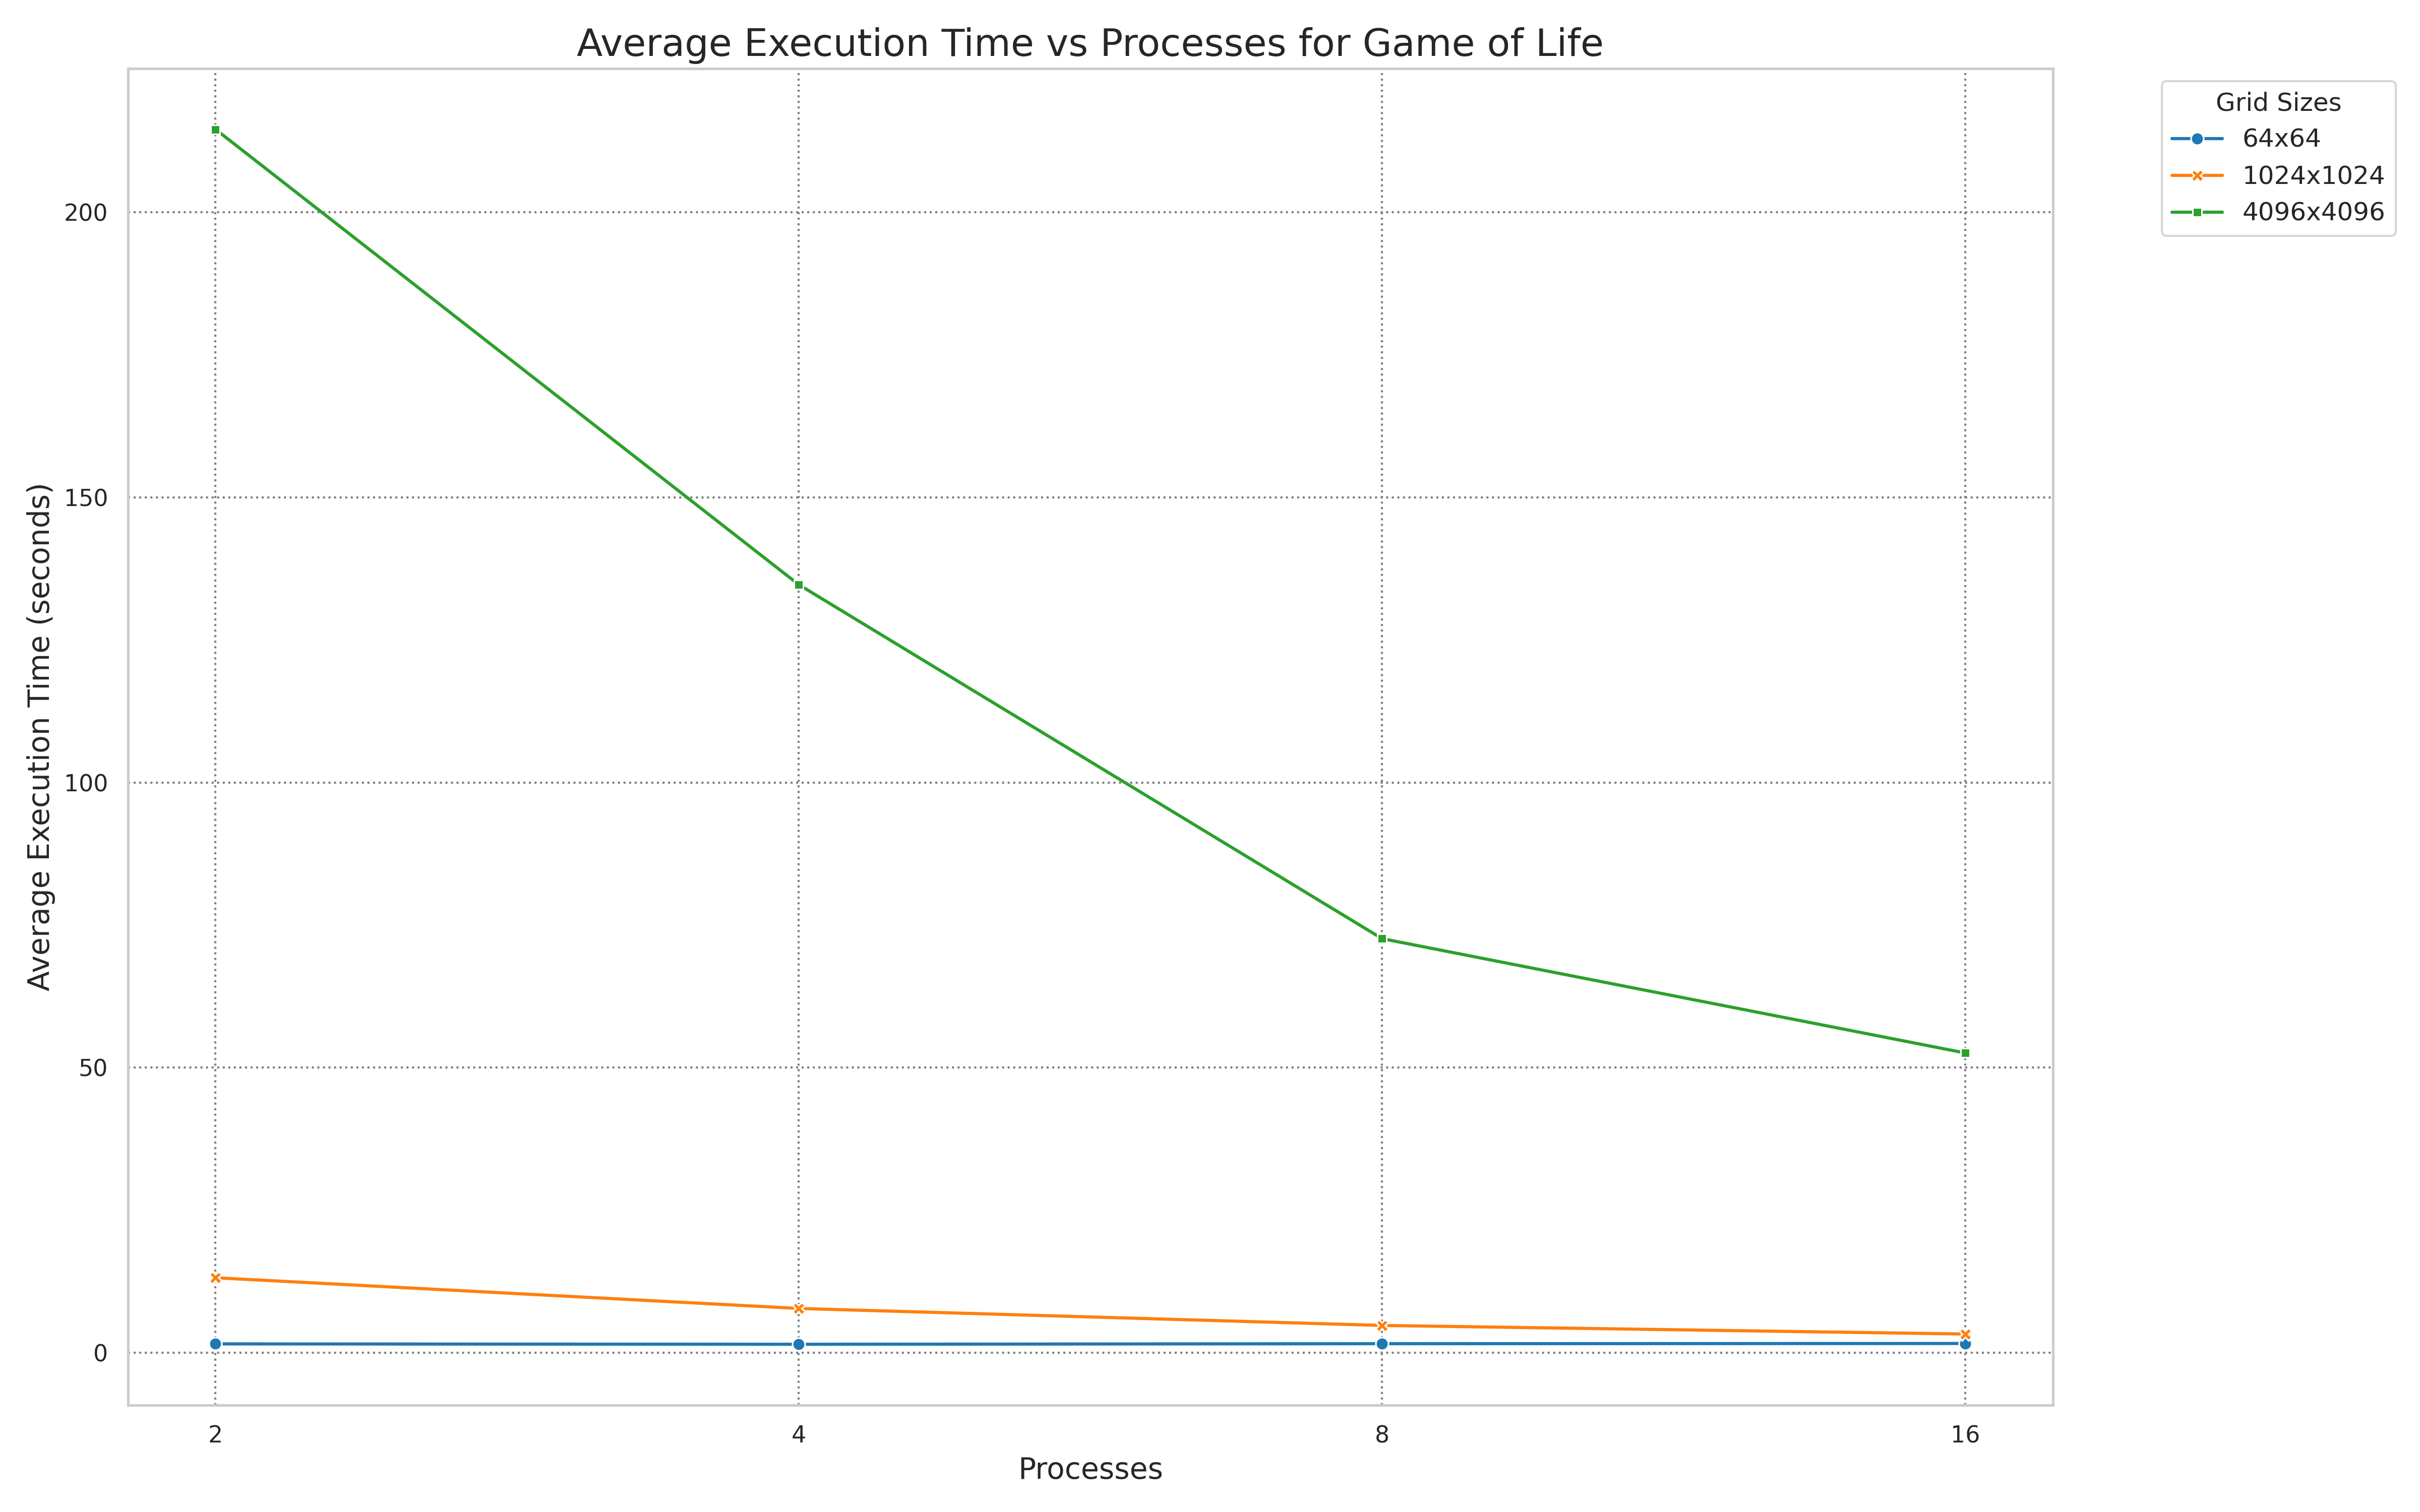
\includegraphics[width=0.8\textwidth]{game_of_life_recv_results.png}
    \caption{Χρόνοι εκτέλεσης για το Παιχνίδι της Ζωής με Recv-Isend}
\end{figure}
\subsection*{Συμπεράσματα}
Η χρήση ασύγχρονων επικοινωνιών στο Παιχνίδι της Ζωής με MPI οδηγεί σε σημαντική βελτίωση της απόδοσης, ειδικά για μικρά και μεσαία μεγέθη πλέγματος. Για μεγάλα πλέγματα, η βελτίωση είναι αισθητή, αλλά όχι τόσο σημαντική. Η επιλογή της βέλτιστης στρατηγικής επικοινωνίας εξαρτάται από το μέγεθος του προβλήματος και τον αριθμό των διεργασιών. Η χρονική επικάλυψη αποδεικνύεται ιδιαίτερα αποτελεσματική όταν ο χρόνος επικοινωνίας είναι υψηλός σε σχέση με τον χρόνο υπολογισμού, όπως συμβαίνει σε μικρά πλέγματα
\section*{Άσκηση 3.4}
\subsection*{Εισαγωγή}
Στην Άσκηση 3.4, τροποποιήθηκε το πρόγραμμα της Άσκησης 3.1 ώστε να χρησιμοποιεί υβριδικά το MPI (για την εκμετάλλευση της παραλληλίας μεταξύ των κόμβων) και το OpenMP (για την εκμετάλλευση της παραλληλίας των πυρήνων μέσα σε κάθε κόμβο). Ο στόχος ήταν να συγκρίνουμε την απόδοση αυτής της υβριδικής υλοποίησης με την υλοποίηση που βασίζεται αποκλειστικά στο MPI, διατηρώντας τη συνολική χρήση πόρων (κόμβοι και πυρήνες ανά κόμβο) σταθερή.
\subsection*{Συγχρονισμός}
Ο συγχρονισμός μεταξύ των διεργασιών MPI γίνεται μέσω των \texttt{\path{MPI_Scatter}}, \texttt{\path{MPI_Sendrecv}}, και \texttt{\path{MPI_Gather}}. Η \texttt{\path{MPI_Scatter}} χρησιμοποιείται για την κατανομή του πλέγματος στις διεργασίες, η \texttt{\path{MPI_Sendrecv}} για την ανταλλαγή γραμμών ορίων (ghost rows) μεταξύ γειτονικών διεργασιών, και η \texttt{\path{MPI_Gather}} για τη συλλογή των αποτελεσμάτων από όλες τις διεργασίες. Αυτές οι λειτουργίες εξασφαλίζουν ότι οι διεργασίες συνεργάζονται αποτελεσματικά και ότι τα δεδομένα παραμένουν συνεπή κατά τη διάρκεια της εκτέλεσης.
\subsection*{Πειραματική Διαδικασία}
\begin{itemize}
    \item \textbf{Παραμετροποίηση:}
    \begin{itemize}
        \item Μέγεθος πλέγματος: $64\times64$, $1024\times1024$.
        \item Αριθμός διεργασιών MPI: 2, 4, 8, 16.
        \item Αριθμός γενιών: 1000.
        \item Αριθμός πυρήνων ανά κόμβο: 4 (σταθερός για όλα τα πειράματα).
    \end{itemize}
    \item \textbf{Εκτέλεση:}
    \begin{itemize}
        \item Τα πειράματα εκτελέστηκαν 5 φορές για κάθε συνδυασμό παραμέτρων.
        \item Καταγράφηκε ο χρόνος εκτέλεσης για κάθε πείραμα.
        \item Τα δεδομένα αποθηκεύτηκαν σε CSV αρχείο.
    \end{itemize}
    \item \textbf{Αυτοματοποίηση:}
    \begin{itemize}
        \item Αναπτύχθηκαν Python scripts για την εκτέλεση των πειραμάτων και την καταγραφή των δεδομένων.
        \item Χρησιμοποιήθηκαν Python scripts για την επεξεργασία των αποτελεσμάτων και τη δημιουργία γραφημάτων.
    \end{itemize}
\end{itemize}
\subsection*{Αποτελέσματα}
Από τα αποτελέσματα των μετρήσεων, παρατηρούμε τα εξής:
\begin{enumerate}
    \item \textbf{Για μικρά μεγέθη πλέγματος (64x64)}:
    \begin{itemize}
        \item Η υβριδική υλοποίηση (MPI + OpenMP) έχει σημαντικά μεγαλύτερους χρόνους εκτέλεσης σε σύγκριση με την υλοποίηση που βασίζεται αποκλειστικά στο MPI. Για παράδειγμα, για 2 διεργασίες, ο μέσος χρόνος εκτέλεσης για την υβριδική υλοποίηση είναι 44.34903 s, ενώ για την MPI υλοποίηση είναι 1.72495 s.
    \end{itemize}
    \item \textbf{Για μεσαία μεγέθη πλέγματος (1024x1024)}:
    \begin{itemize}
        \item Στην περίπτωση των 8 διεργασιών, η υβριδική υλοποίηση (325.04016 s) είναι πιο αργή από την καθαρά MPI υλοποίηση (22.11091 s). Αυτό οφείλεται στο γεγονός ότι το κόστος της διαχείρισης των νημάτων OpenMP και η επικοινωνία μεταξύ των διεργασιών MPI είναι υψηλό, χωρίς να αντισταθμίζεται από την παράλληλη εκτέλεση των πυρήνων.
    \end{itemize}
\end{enumerate}
\subsection*{Γραφήματα}
\newpage
\begin{figure}[h]
    \centering
    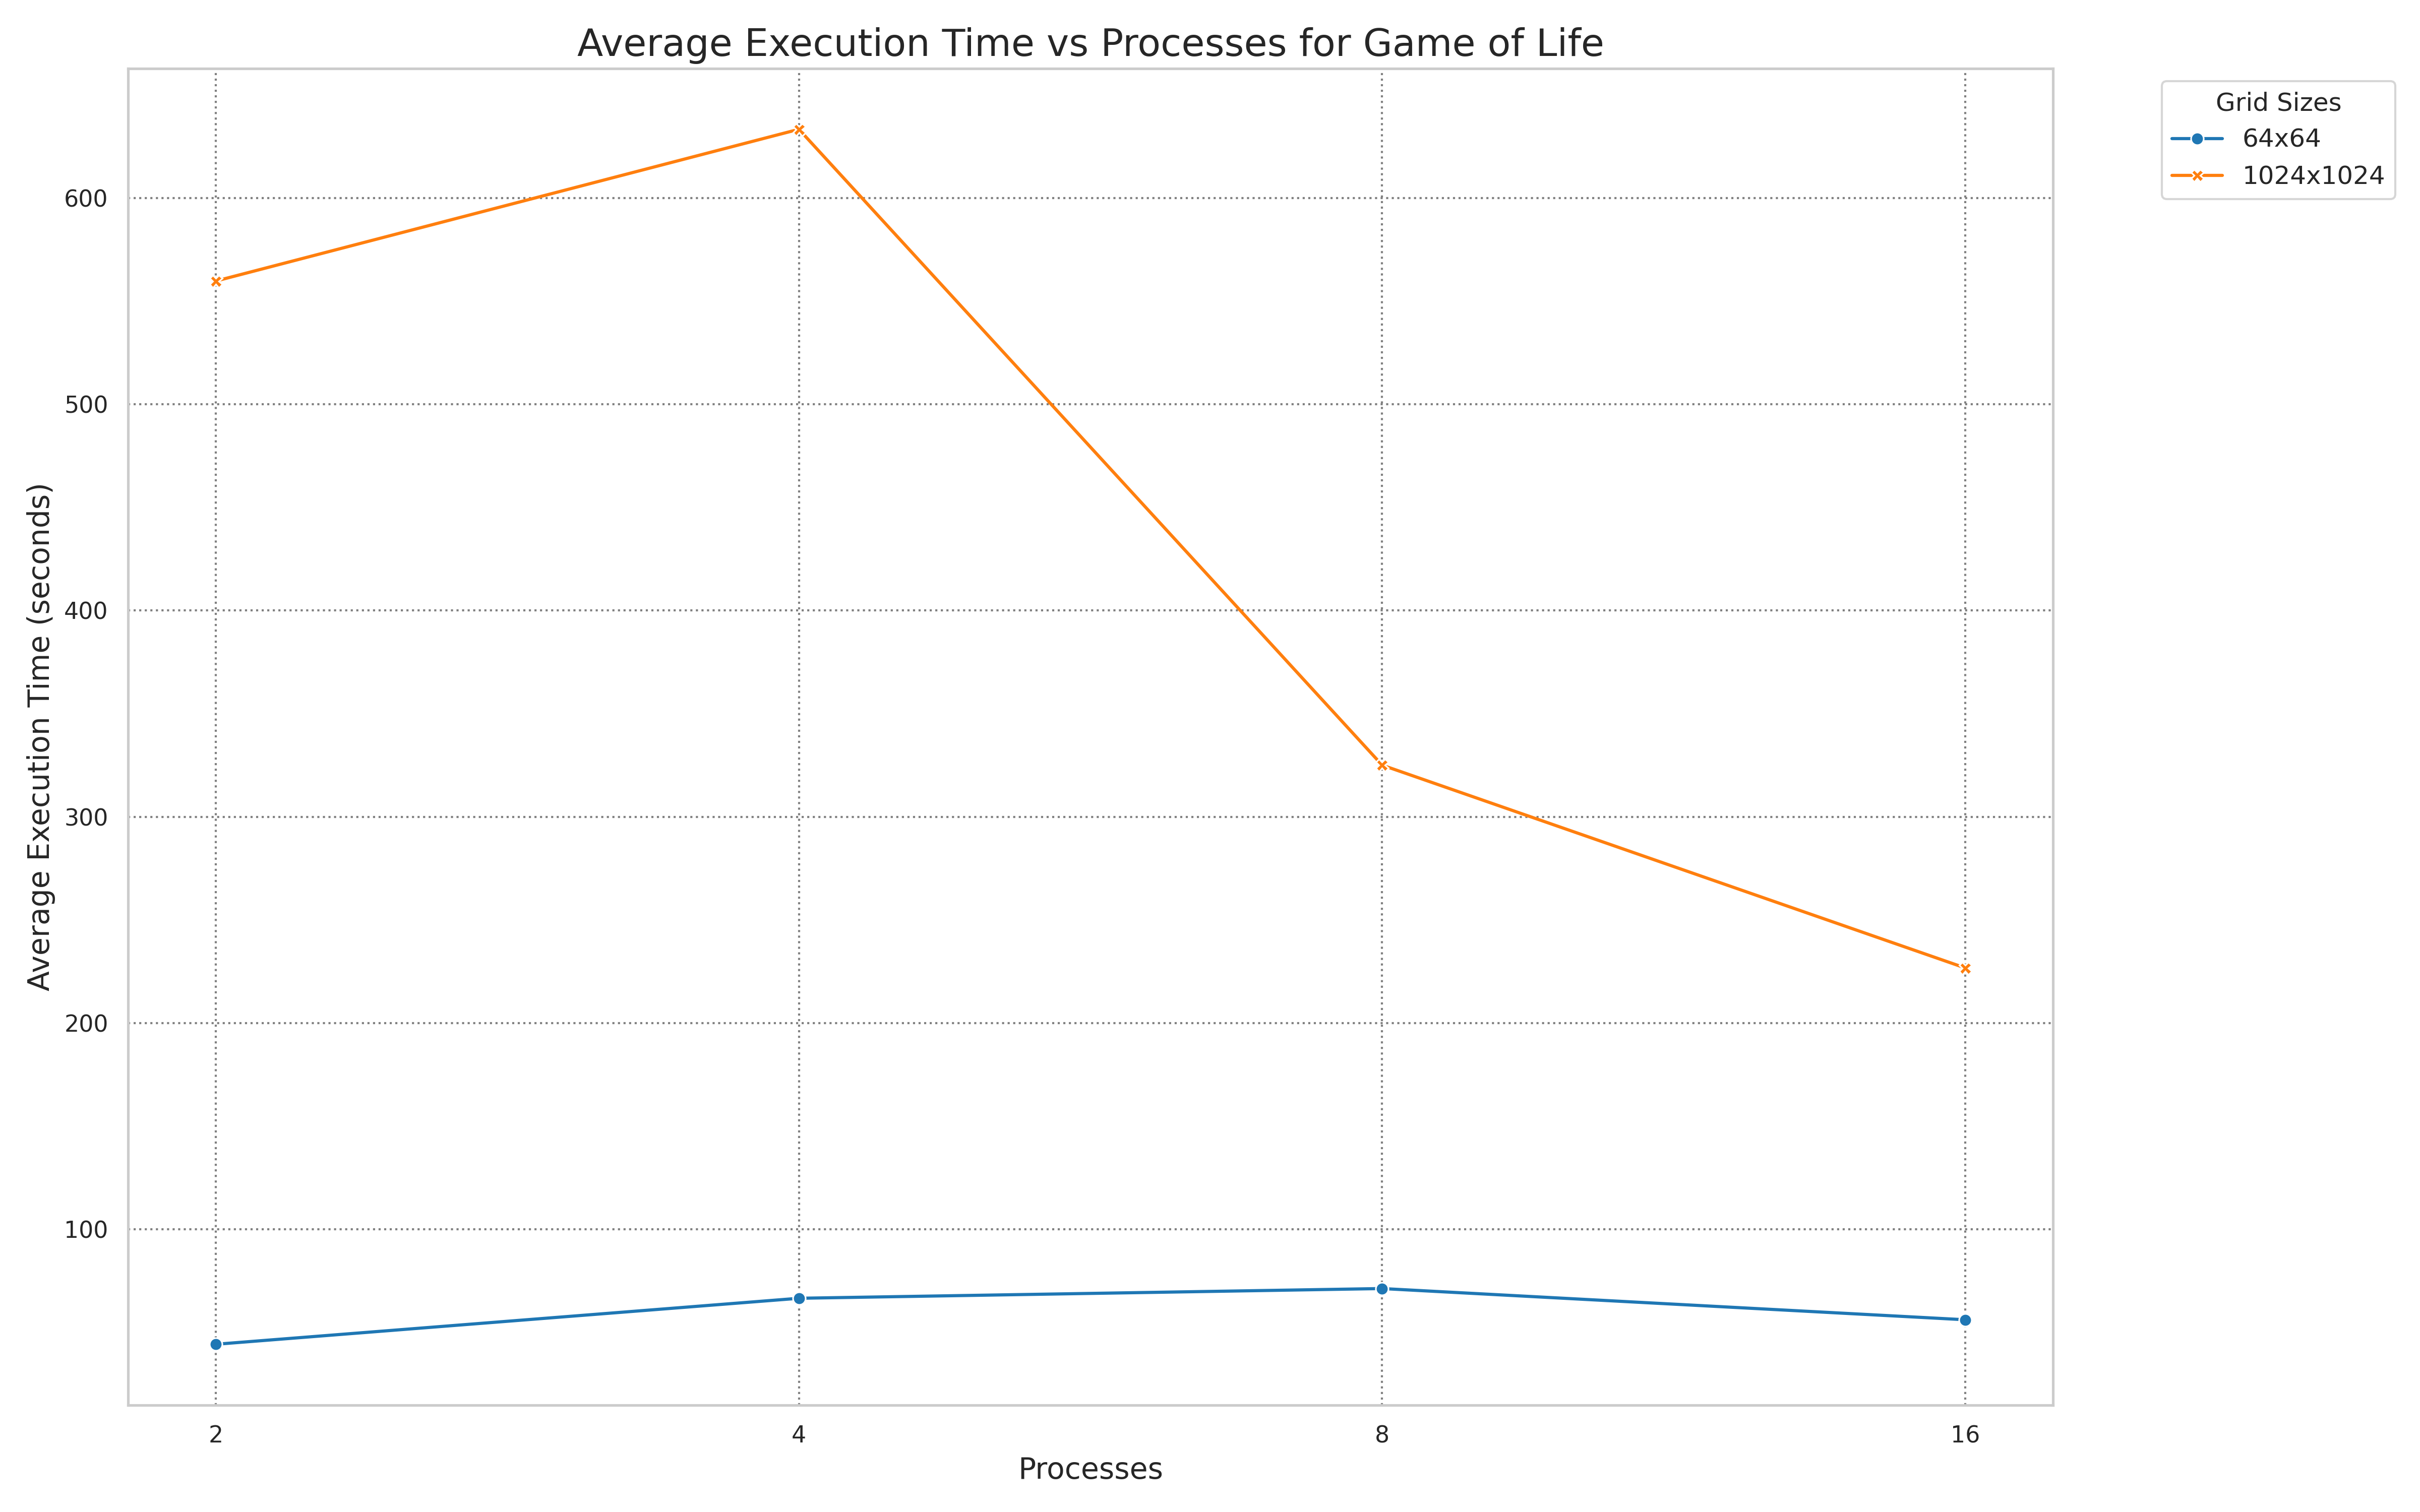
\includegraphics[width=0.8\textwidth]{game_of_life_hybrid_results.png}
    \caption{Χρόνοι εκτέλεσης για το Παιχνίδι της Ζωής με Υβριδική Υλοποίηση}
\end{figure}
\subsection*{Συμπεράσματα}
Από τα αποτελέσματα και τα γραφήματα, μπορούμε να εξάγουμε τα εξής συμπεράσματα:
\begin{enumerate}
    \item \textbf{Επίδραση του μεγέθους πλέγματος}:
    \begin{itemize}
        \item Για μικρά μεγέθη πλέγματος, η υβριδική υλοποίηση δεν προσφέρει σημαντική βελτίωση στην απόδοση, καθώς το κόστος της διαχείρισης των νημάτων OpenMP είναι υψηλό σε σχέση με τον χρόνο υπολογισμού.
        \item Για μεγαλύτερα πλέγματα, η υβριδική υλοποίηση μπορεί να γίνει πιο αποτελεσματική, αλλά στα αποτελέσματά παρατηρείται ότι για το πλέγμα 1024x1024, η υβριδική υλοποίηση ήταν πιο αργή από την καθαρά MPI υλοποίηση. Αυτό υποδηλώνει ότι η χρήση του OpenMP δεν ήταν αποτελεσματική για αυτό το μέγεθος πλέγματος.
    \end{itemize}
        \item \textbf{Επίδραση του αριθμού των διεργασιών}:
    \begin{itemize}
        \item Για μικρά πλέγματα, η αύξηση του αριθμού των διεργασιών οδηγεί σε αύξηση του χρόνου εκτέλεσης λόγω του κόστους επικοινωνίας και της διαχείρισης των νημάτων OpenMP.
        \item Για μεγάλα πλέγματα, η αύξηση του αριθμού των διεργασιών οδηγεί σε σημαντική μείωση του χρόνου εκτέλεσης, καθώς ο χρόνος υπολογισμού είναι πολύ μεγαλύτερος από το κόστος επικοινωνίας και τη διαχείριση των νημάτων.
    \end{itemize}
        \item \textbf{Βέλτιστος αριθμός διεργασιών}:
    \begin{itemize}
        \item Για κάθε μέγεθος πλέγματος, υπάρχει ένας βέλτιστος αριθμός διεργασιών που εξαρτάται από το μέγεθος του πλέγματος, το κόστος επικοινωνίας και τη διαχείριση των νημάτων OpenMP. Για παράδειγμα, για πλέγμα 1024x1024, η καθαρά MPI υλοποίηση με 4 διεργασίες φαίνεται να είναι η πιο αποτελεσματική, με μέσο χρόνο εκτέλεσης 7.71714 s.
    \end{itemize}
\end{enumerate}
Συνολικά, η υβριδική υλοποίηση του Παιχνιδιού της Ζωής με MPI και OpenMP δεν φαίνεται να προσφέρει σημαντική βελτίωση στην απόδοση για τα μεγέθη πλέγματος που δοκιμάστηκαν. Για μικρά και μεσαία πλέγματα, η καθαρά MPI υλοποίηση φαίνεται να είναι πιο αποτελεσματική. Η επιλογή του βέλτιστου αριθμού διεργασιών και νημάτων εξαρτάται από το μέγεθος του πλέγματος και το κόστος επικοινωνίας μεταξύ των διεργασιών
\end{document}